%! suppress = LineBreak
\documentclass{article}

\usepackage{fancyhdr}
\usepackage{minted}
\usepackage{amsmath}
\usepackage{hyperref}
\usepackage{array}
\usepackage{booktabs} % For cleaner tables (optional)
\usepackage{graphicx}
\usepackage[table,xcdraw]{xcolor}
\usepackage{caption}
\usepackage{listings}

\lstset{
    breaklines=true,
    breakatwhitespace=true,
    basicstyle=\ttfamily,
    columns=fullflexible
}

\usepackage[sorting=none,backend=biber]{biblatex}
\usepackage[
    a4paper,
    left=0.75in,
    right=0.75in,
    top=0.75in,
    bottom=0.75in
]{geometry}
\usepackage{mathtools}
\usepackage{blindtext}
\addbibresource{BamFeatures.bib}


\hypersetup{
    colorlinks=true,   % Farben statt Umrandung für Links
    linkcolor=black,    % Farbe für interne Links
    citecolor=blue,    % Farbe für Zitate
    filecolor=blue,    % Farbe für Dateien
    urlcolor=blue      % Farbe für URLs
}


\pagestyle{fancy}
\title{Topic 4: Differential Analysis\\\large Lab Course Genome-Oriented Bioinformatics}
\author{}
\date{20.01.2025}


\begin{document}

    \maketitle
    \renewcommand{\abstractname}{}
    \begin{abstract}
        \large
    \end{abstract}
    \hrule
    \tableofcontents
    \vspace{10pt} % Optional: Add space after the TOC as well
    \hrule


    \section{Introduction}\label{sec:introduction}

    \begin{figure}[!htpb]
        \centering
        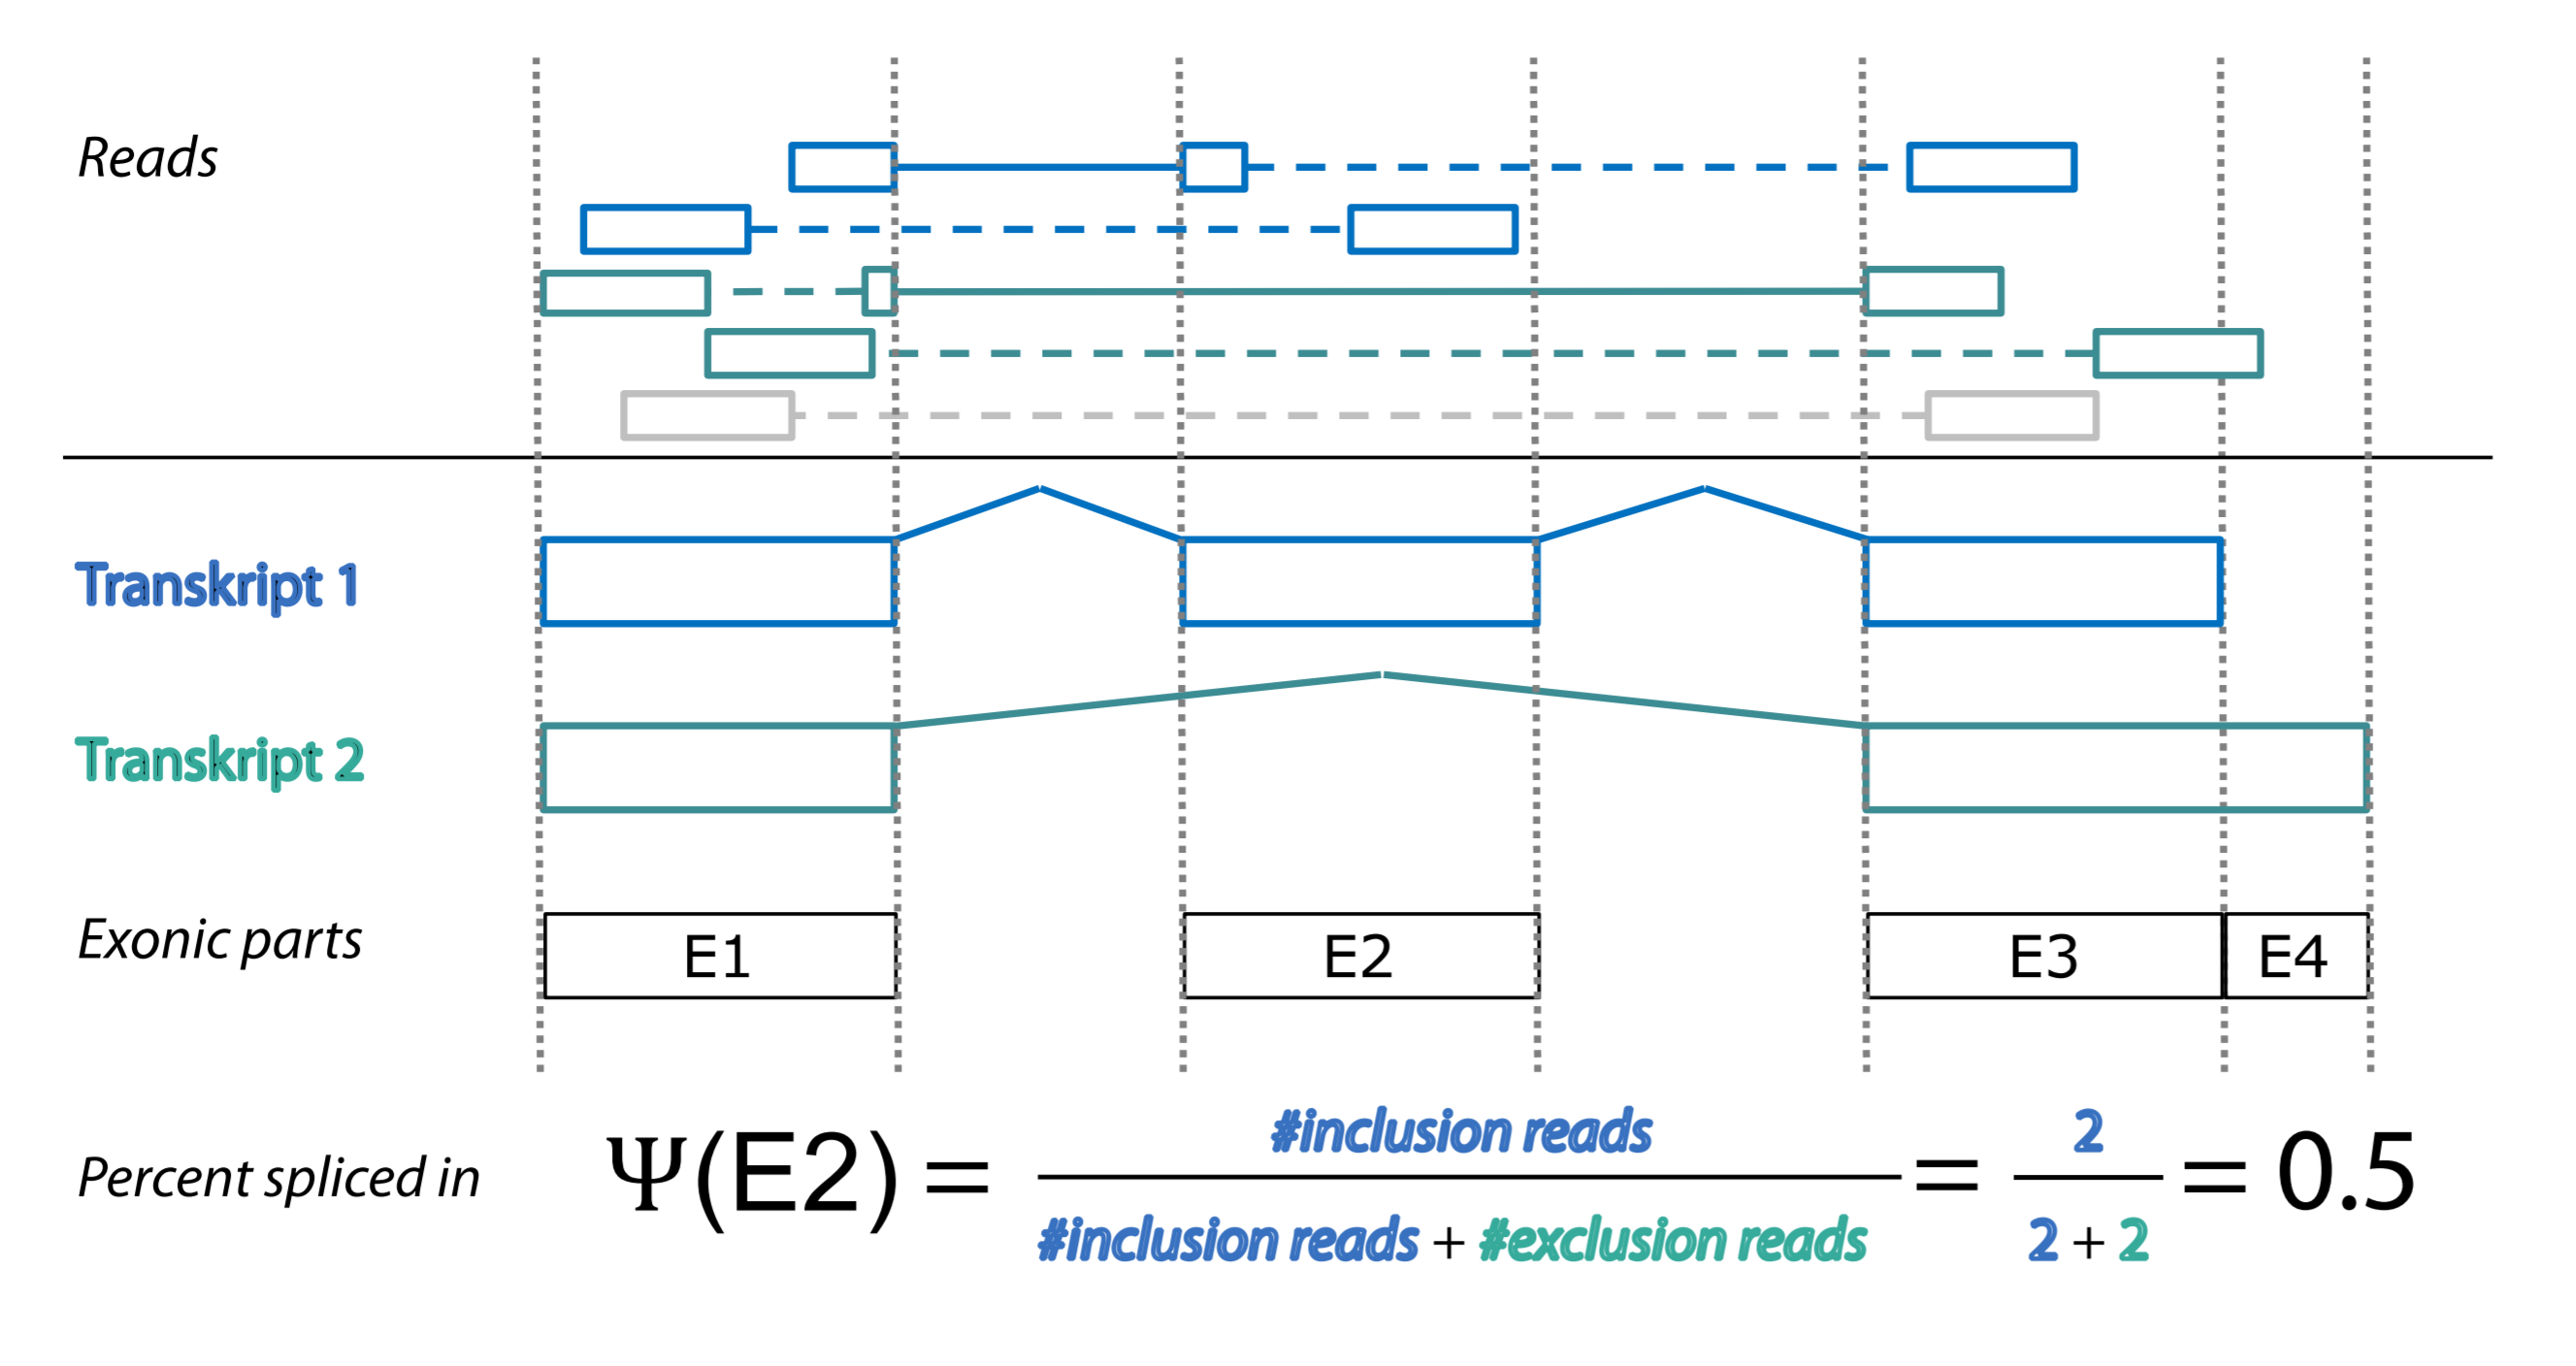
\includegraphics[width=0.7\textwidth]{figures/alternativesplicing/example_exon_skipping_event}
        \caption
        {Diagram showing an example exon skipping event and which reads are considered as included, excluded, or ambiguous for the PSI calculation. Transcript 1 would be the wild type, while Transcript 2 would be the splicing variant. Exon 2 is skipped in Transcript 2.}
        \label{fig:example-exon-skipping-event}
    \end{figure}

    \begin{figure}[h]
        \centering
        \begin{equation}
            \Psi (E) = \frac{I}{I+E}
            \label{eq:psi}
        \end{equation}
        \caption{$\Psi$ value for a given exon $E$ is calculated by dividing the number of included reads $I$ by the sum of included and excluded reads $I+E$.}
    \end{figure}


    \section{Materials and Methods}\label{sec:materials-and-methods}

    \subsection{Compute Percent-Spliced-In (PSI) values}\label{subsec:compute-percent-spliced-in-(psi)-values}
    Figure \ref{fig:alternative-splicing-process} shows the general process for solving the BamFeatures assignment. Due to the complexity of this assignment and the numerous cases, a flowchart is optimal for understanding the task. This allows optimal structuring of an implementation, as one can see which checks can be performed first, in order to possibly rule out other checks from needing to be made, saving computation time. The flowchart shows the process of processing a single read but differs from the actual implementation due to structural reasons. This is because the implementation processes the reads in batches (by chromosome), instead of one by one. The general structure of the program is described below:
    \begin{enumerate}
        \item \textbf{Initialization and Setup}: Creation of the \texttt{AlternativeSplicingAnnotator} object which initializes the \texttt{GTFAnnotation}, calculates the exon skipping events (as per the first report), as well as initializing the \texttt{SamReader}, and \texttt{IntervalTreeForestManager}.
        \item \textbf{Iteration Process}:
        \begin{enumerate}
            \item \textbf{Iterate through the SamReader}: Iterate to the next record, unless the end of the file is reached in which case go to step \ref{sec:last-chromosome-processing} \label{sec:iterate-samreader}
            \item \textbf{Chromosome Check}: Check if the current record is on the same chromosome as the previous record. If not, process the reads in step \ref{sec:new-chromosome-processing}. \label{sec:chromosome-check}
            \item \textbf{Valid Read Check}: Check conditions if the read is valid. If not, continue to step \ref{sec:iterate-samreader}.
            \item \textbf{Read Pair Check}: Check if we have seen the record's mate before:
            \begin{itemize}
                \item If yes, add the records in the correct order (first of pair) to the readsToAnnotate List
                \item If no, add the record to the lookup table and continue to the next record.
            \end{itemize}
            \item Go to step \ref{sec:iterate-samreader}.
        \end{enumerate}
        \item \textbf{New Chromosome Processing} \label{sec:new-chromosome-processing}:
        \begin{enumerate}
            \item \textbf{Read Processing}: \label{sec:read-processing}
            \begin{enumerate}
                \item Calculate the Read's attributes such as the combined read intervals, extracting alignmen start and end, etc.
                \item If there are any \texttt{cgenes}, check for a transcriptomic match.
                \item For each matched gene with a transcriptomic match, iterate through the
            \end{enumerate}
            \item Reset the data structures and return to step \ref{sec:chromosome-check}.
        \end{enumerate}
        \item \textbf{Last Chromosome Processing} \label{sec:last-chromosome-processing}:
        \begin{enumerate}
            \item Process the reads like in Step \ref{sec:read-processing}. Close the writer.
        \end{enumerate}
    \end{enumerate}

    \subsubsection{Program Usage}
    \begin{verbatim}
usage: java -jar differentialanalysis.jar [-h] -gtf <gtf_file> -bam <bamfile> -o <output_tsv>
named arguments:
  -h, --help             show this help message and exit
  -gtf <gtf_file>        GTF file
  -bam <bamfile>         BAM file
  -o <output_tsv>        Output file
    \end{verbatim}

    \begin{figure}[!htpb]
        \centering
        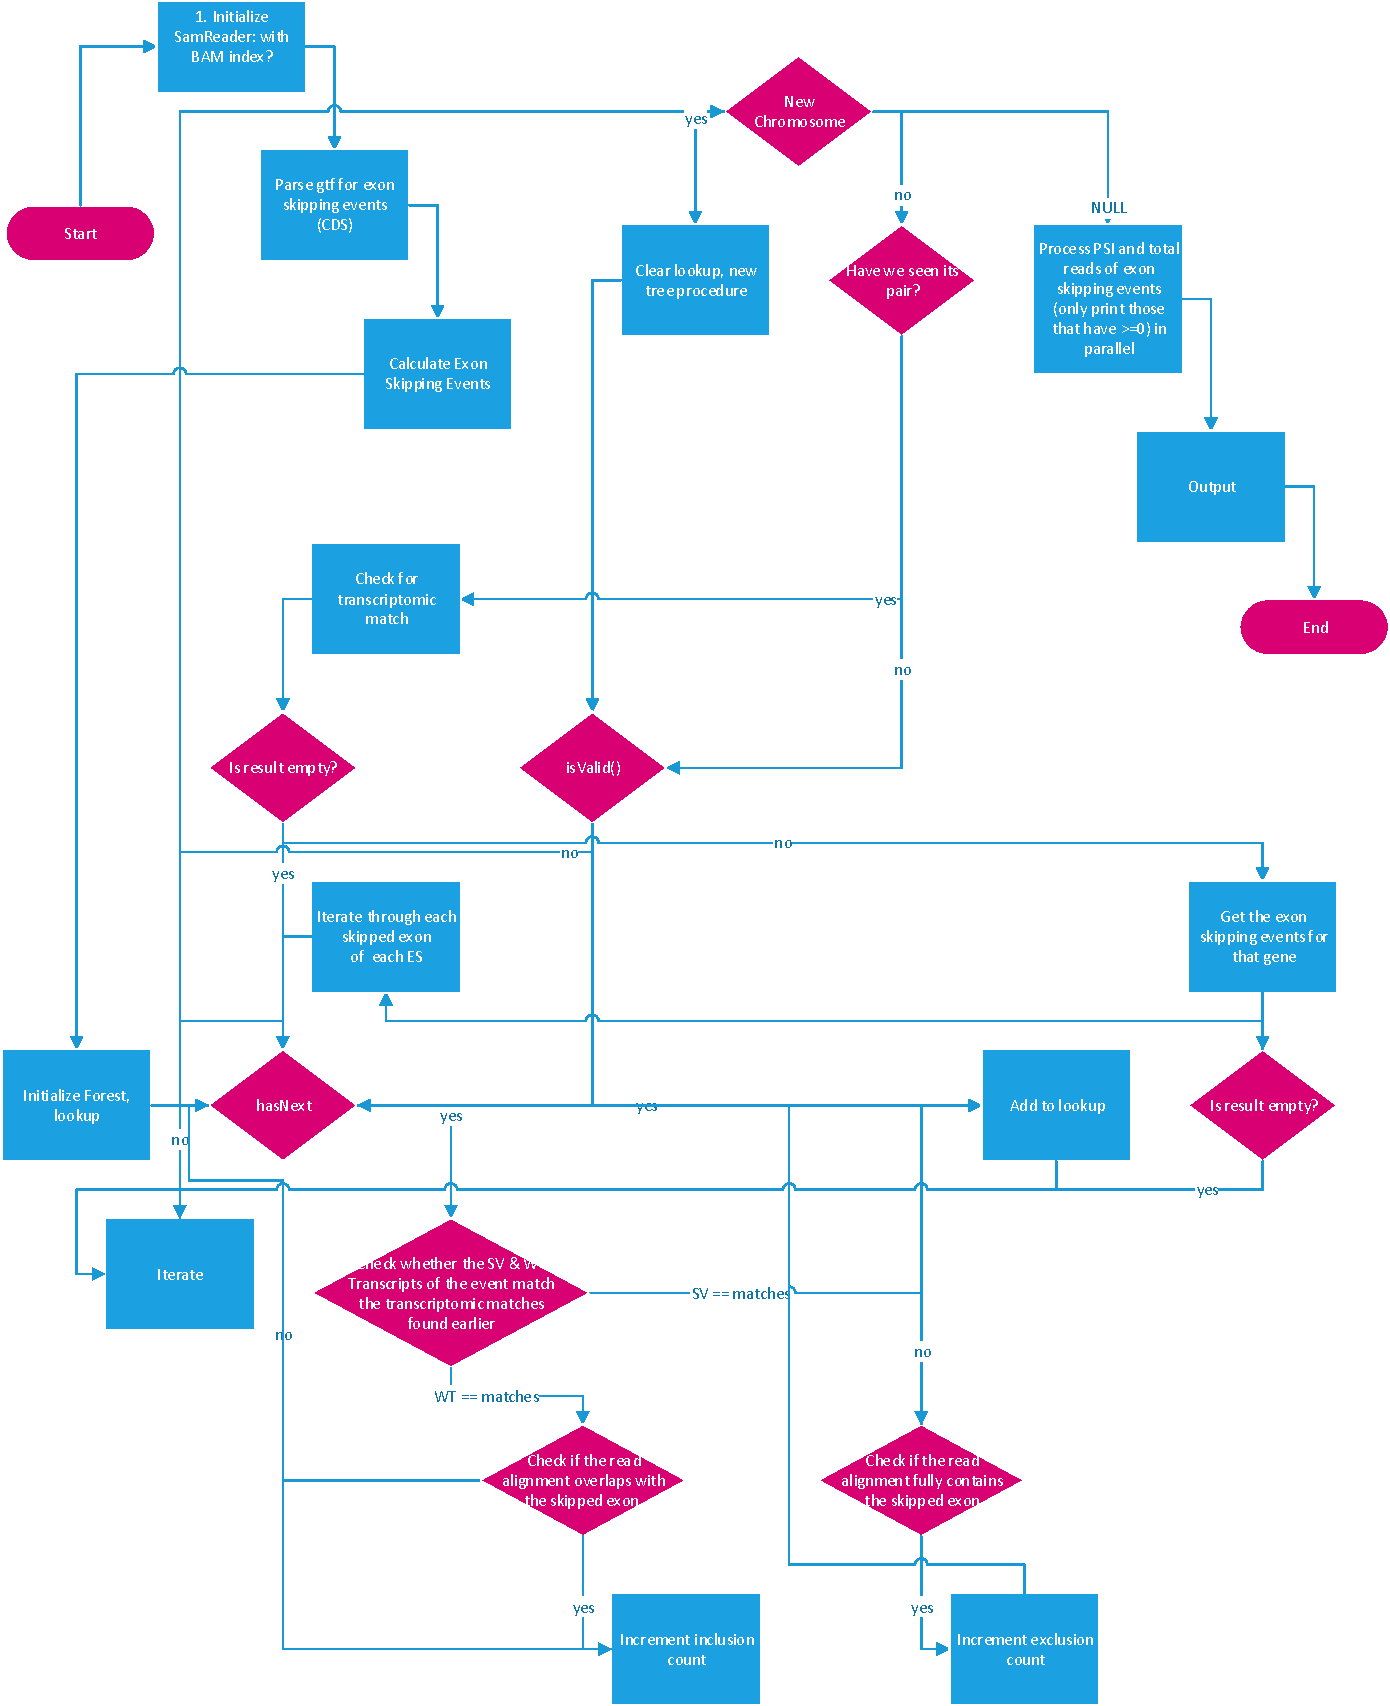
\includegraphics[width=0.7\textwidth]{figures/alternativesplicing/AlternativeSplicingProcess-crop}
        \caption
        {Flowchart illustrating the logical program flow for solving the Alternative Splicing Assignment. Rectangles represent procedures, diamonds represent decisions,
            and rounded blocks represent start and endpoints. The process involves parsing the GTF, calculating the exon skipping events and iterating through the BAMFile. Once both forward and reverse reads have been found,
            the processing is performed.}
        \label{fig:alternative-splicing-process}
    \end{figure}

    \subsection{Simple differential test of PSI-values}\label{subsec:simple-differential-test-of-psi-values}
    Comparison with other alternative splicing tools (DEXSeq)
    \subsection[Alternative Splicing Comparison]{Comparison With Other Alternative Splicing Tools}\label{subsec:comparison-with-other-alternative-splicing-tools}


    \section{Analysis}\label{sec:analysis}


    \section{Supplement}\label{sec:supplement}

    \pagebreak
\end{document}
